% !TEX root = ../../../proposal.tex

%\begin{abstract}
We investigate the security of Diffie-Hellman key exchange as used in popular
Internet protocols and find it to be less secure than widely believed. First,
we present Logjam, a novel flaw in TLS that lets a man-in-the-middle
downgrade connections to ``export-grade'' Diffie-Hellman. To carry out this
attack, we implement the number field sieve discrete log algorithm. After a
week-long precomputation\footnote{\small Except where otherwise noted, the
experimental data and network measurements for this article were obtained in
early 2015.} for a specified 512-bit group, we can compute arbitrary discrete
logs in that group in about a minute. We find that 82\% of vulnerable servers
use a single 512-bit group, allowing us to compromise connections to 7\% of
Alexa Top Million HTTPS sites. In response, major browsers have changed to
reject short groups.
%\looseness=-1

We go on to consider Diffie-Hellman with 768- and 1024-bit groups. We
estimate that even in the 1024-bit case, the computations are plausible given
nation-state resources. A small number of fixed or standardized groups are
used by millions of servers; performing precomputation for a single 1024-bit
group would allow passive eavesdropping on 18\% of popular HTTPS sites, and a
second group would allow decryption of traffic to 66\% of IPsec VPNs and 26\%
of SSH servers. A close reading of published NSA leaks shows that the
agency's attacks on VPNs are consistent with having achieved such a break. We
conclude that moving to stronger key exchange methods should be a priority
for the Internet community.
%\looseness=-1
%\end{abstract}

\section{Introduction}

Diffie-Hellman key exchange is a popular cryptographic algorithm that allows
Internet protocols to agree on a shared key and negotiate a secure
connection. It is fundamental to protocols such as HTTPS, SSH, IPsec, SMTPS,
and other protocols that rely on TLS\@. Many protocols use Diffie-Hellman to
achieve \emph{perfect forward secrecy}, the property that a compromise of the
long-term keys used for authentication does not compromise sessions keys for
past connections. We examine how Diffie-Hellman is commonly implemented and
deployed with common protocols and find that, in practice, it frequently
offers less security than widely believed.

There are two reasons for this. First, a surprising number of servers use
weak Diffie-Hellman parameters or maintain support for obsolete 1990s-era
``export-grade'' crypto. More critically, the common practice of using
standardized, hard-coded, or widely shared Diffie-Hellman parameters has the
effect of dramatically reducing the cost of large-scale attacks, bringing
some within range of feasibility today.

The current best technique for attacking Diffie-Hellman relies on
compromising one of the private exponents ($a$, $b$) by computing the
discrete logarithm of the corresponding public value ($g^a \bmod p$, $g^b
\bmod p$). With state-of-the-art number field sieve algorithms, computing a
single discrete log is more difficult than factoring an RSA modulus of the
same size. However, an adversary who performs a large precomputation for a
prime $p$ can then quickly calculate arbitrary discrete logs in that group,
amortizing the cost over all targets that share this parameter. Although this
fact is well known among mathematical cryptographers, it seems to have been
lost among practitioners deploying cryptosystems. We exploit it to
obtain the following results:

\paragraph{Active attacks on export ciphers in TLS}
We introduce Logjam, a new attack on TLS by which a man-in-the-middle
attacker can downgrade a connection to export-grade cryptography. This attack
is reminiscent of the FREAK attack~\cite{freak-attack-2015} but applies to
the ephemeral Diffie-Hellman ciphersuites and is a TLS protocol flaw rather
than an implementation vulnerability. We present measurements that show that
this attack applies to 8.4\% of Alexa Top Million HTTPS sites and 3.4\% of
all HTTPS servers that have browser-trusted certificates.

To exploit this attack, we implemented the number field sieve discrete log
algorithm and carried out precomputation for two 512-bit Diffie-Hellman
groups used by more than 92\% of the vulnerable servers. This allows us to
compute individual discrete logs in about a minute. Using our discrete log
oracle, we can compromise connections to over 7\% of Top Million HTTPS sites.
Discrete logs over larger groups have been computed before~\cite{dlp180},
but, as far as we are aware, this is the first time they have been exploited
to expose concrete vulnerabilities in real-world systems.
%\looseness=-1


\begin{figure*}[ht]
\centering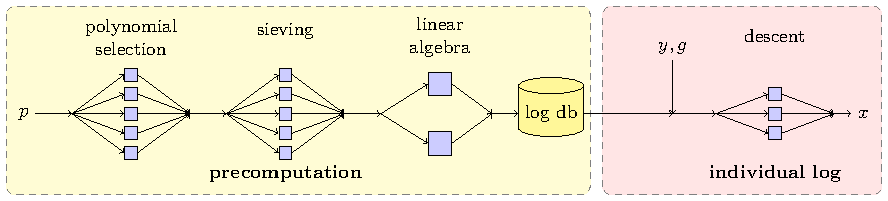
\includegraphics[width=\linewidth]{\LogjamFigures/nfs}

\caption{\textbf{Number field sieve for discrete log}\,---\,%
This algorithm consists of a precomputation stage that depends only on the
prime $p$ and a descent stage that computes individual logarithms. With
sufficient precomputation, an attacker can quickly break any Diffie-Hellman
instances that use a particular $p$.
}
\label{fig:nfs}
\end{figure*}

\paragraph{Risks from common 1024-bit groups}
We explore the implications of precomputation attacks for 768- and 1024-bit
groups, which are widely used in practice and still considered secure. We
estimate the computational resources necessary to compute discrete logs in
groups of these sizes, concluding that 768-bit groups are within range of
academic teams, and 1024-bit groups may plausibly be within range of
nation-state adversaries. In both cases, individual logarithms can be quickly
computed after the initial precomputation.

We then examine evidence from published Snowden documents that suggests NSA
may already be exploiting 1024-bit Diffie-Hellman to decrypt VPN traffic. We
perform measurements to understand the implications of such an attack for
popular protocols, finding that an attacker who could perform precomputations
for ten 1024-bit groups could passively decrypt traffic to about 66\% of IKE
VPNs, 26\% of SSH servers, and 24\% of popular HTTPS sites.

\paragraph{Mitigations and lessons}
In response to the Logjam attack, mainstream browsers have implemented a more
restrictive policy on the size of Diffie-Hellman groups they accept, and
Chrome has discontinued support for finite field key exchanges. We further
recommend that TLS servers disable export-grade cryptography and carefully
vet the Diffie-Hellman groups they use. In the longer term, we advocate that
protocols migrate to elliptic curve Diffie-Hellman.

\section{Diffie-Hellman Cryptanalysis}
\label{sec:dl}

Diffie-Hellman key exchange was the first published public-key
algorithm~\cite{new-directions-in-crypto-1976}. In the simple case of prime
groups, Alice and Bob agree on a prime $p$ and a generator $g$ of a
multiplicative subgroup modulo $p$. Then each generates a random private
exponent, $a$ and $b$. Alice sends $g^a \bmod p$, Bob sends $g^b \bmod p$,
and each computes a shared secret $g^{ab} \bmod p$. While there is also a
Diffie-Hellman exchange over elliptic curve groups, we address only the ``mod
$p$'' case.

The security of Diffie-Hellman is not known to be equivalent to the discrete
logarithm problem, but computing discrete logs remains the best known
cryptanalytic attack. An attacker who can find the discrete log $x$ from $y =
g^x \bmod p$ can easily find the shared secret.

Textbook descriptions of discrete log can be misleading about the
computational tradeoffs, for example by optimizing for computing a
\emph{single} discrete log. In fact, as illustrated in Figure~\ref{fig:nfs},
a single large precomputation on $p$ can be used to efficiently break
\emph{all} Diffie-Hellman exchanges made with that prime.

Diffie-Hellman is typically implemented with prime fields and large group
orders. In this case, the most efficient discrete log algorithm is the number
field sieve
(NFS)~\cite{discrete-log-nfs-1993,virtual-logarithms-2005,nfs-prime-field-2003}.
The algorithm has four stages with different computational properties. The
first three steps are only dependent on the prime $p$ and comprise most of
the computation.

First is \emph{polynomial selection}, in which one finds a polynomial $f(z)$
defining a number field $\QQ[z]/f(z)$ for the computation. This parallelizes
well and is only a small portion of the runtime.

In the second stage, \emph{sieving}, one factors ranges of integers and
number field elements in batches to find many relations of elements, all of
whose prime factors are less than some bound $B$ (called $B$-smooth). Sieving
parallelizes well, but is computationally expensive, because we must search
through and attempt to factor many elements.

In the third stage, \emph{linear algebra}, we construct a large, sparse
matrix consisting of the coefficient vectors of prime factorizations we have
found. This stage can be parallelized in a limited fashion, and produces a
database of logarithms which are used as input to the final stage.

The final stage, \emph{descent}, actually deduces the discrete log of the
target $y$. We re-sieve until we find a set of relations that allow us to
write the logarithm of $y$ in terms of the logarithms in the precomputed
database. Crucially, descent is the only NFS stage that involves $y$ (or
$g$), so polynomial selection, sieving, and linear algebra can be done once
for a prime $p$ and reused to compute the discrete logs of many targets.

The numerous parameters of the algorithm allow some flexibility to reduce
time on some computational steps at the expense of others. For example,
sieving more will result in a smaller matrix, making linear algebra cheaper,
and doing more work in the precomputation makes the final descent step
easier.

\paragraph{Standard primes}
Generating safe primes\footnote{\small An odd prime $p$ is safe when
$(p-1)/2$ is prime.} can be computationally burdensome, so many
implementations use standardized Diffie-Hellman parameters. A prominent
example is the Oakley groups~\cite{rfc2412}, which give ``safe'' primes of
length 768 (Oakley Group 1), 1024 (Oakley Group 2), and 1536 (Oakley Group
5). These groups were published in 1998 and have been used for many
applications since, including IKE, SSH, Tor, and OTR\@.

When primes are of sufficient strength, there seems to be no
disadvantage to reusing them.  However, widespread reuse of
Diffie-Hellman groups can convert attacks that are at the limits of an
adversary's capabilities into devastating breaks, since it allows the
attacker to amortize the cost of discrete log precomputation among
vast numbers of potential targets.


% !TEX root = paper.tex
\section{Attacking TLS}
\label{sec:tls}

TLS supports Diffie-Hellman as one of several possible key exchange
methods, and prior to public disclosure of the attack, about two-thirds of popular HTTPS sites supported it, most
commonly using 1024-bit primes.  However, a smaller number of servers
also support legacy ``export-grade'' Diffie-Hellman using 512-bit
primes that are well within reach of NFS-based
cryptanalysis. Furthermore, for both normal and export-grade
Diffie-Hellman, the vast majority of servers use a handful of common
groups.

In this section, we exploit these facts to construct a novel attack against
TLS\@, which we call the Logjam attack. First, we perform NFS precomputations
for the two most popular 512-bit primes on the web, so that we can quickly
compute the discrete log for any key exchange message that uses one of them.
Next, we show how a man-in-the-middle, so armed, can attack connections
between popular browsers and any server that allows export-grade
Diffie-Hellman, by using a TLS protocol flaw to downgrade the connection to
export-strength and then recovering the session key. We find that this attack
with our precomputations can compromise connections to about 7.8\% of HTTPS
servers among Alexa Top Million domains.

\begin{table}[t]
	\centering\small
	\begin{tabular}{lll}
          \toprule
          Source  & Popularity & Prime \\
          \midrule
          Apache   & 82\% & \tt 9fdb8b8a004544f0045f1737d0ba2e0b\\
                   &      & \tt 274cdf1a9f588218fb435316a16e3741\\
                   &      & \tt 71fd19d8d8f37c39bf863fd60e3e3006\\
                   &      & \tt 80a3030c6e4c3757d08f70e6aa871033\smallskip\\
          mod\_ssl & 10\% & \tt d4bcd52406f69b35994b88de5db89682\\
                   &      & \tt c8157f62d8f33633ee5772f11f05ab22\\
                   &      & \tt d6b5145b9f241e5acc31ff090a4bc711\\
                   &      & \tt 48976f76795094e71e7903529f5a824b\smallskip\\
          (\emph{others\/}) & \ 8\% & (463~distinct primes) \\
          \bottomrule
	\end{tabular}
    \caption{\textbf{Top 512-bit DH primes for TLS}\,---\,%
        8.4\% of Alexa Top~1M HTTPS domains allow \dheexp{}, of which 92.3\% use
        one of the two most popular primes, shown here.
    }
    \label{tab:export-primes}
\end{table}

\subsection{TLS and Diffie-Hellman}

The TLS handshake begins with a negotiation to determine the crypto
algorithms used for the session. The client sends a list of supported
ciphersuites (and a random nonce $cr$) within the \textsf{ClientHello}
message, where each ciphersuite specifies a key exchange algorithm and other
primitives. The server selects a ciphersuite from the client's list and
signals its selection in a \textsf{ServerHello} message (containing a random
nonce $sr$).

TLS specifies ciphersuites supporting multiple varieties of Diffie-Hellman.
Textbook Diffie-Hellman with unrestricted strength is called ``ephemeral''
Diffie-Hellman, or \dhe{}, and is identified by ciphersuites that begin with
\texttt{TLS\_DHE\_*}.\footnote{\small New ciphersuites that use elliptic
curve Diffie-Hellman (\ecdhe{}) are gaining in popularity, but we focus
exclusively on the traditional prime field variety.} In \dhe{}, the server is
responsible for selecting the Diffie-Hellman parameters. It chooses a group
$(p,g)$, computes $g^b$, and sends a \textsf{ServerKeyExchange} message
containing a signature over the tuple $(cr, sr, p, g, g^b)$ using the
long-term signing key from its certificate. The client verifies the signature
and responds with a \textsf{ClientKeyExchange} message containing $g^a$.

To ensure agreement on the negotiation messages, and to prevent downgrade
attacks, each party computes the TLS master secret from $g^{ab}$ and
calculates a MAC of its view of the handshake transcript. These MACs are
exchanged in a pair of \textsf{Finished} messages and verified by the
recipients.

\paragraph{Export-grade Diffie-Hellman}
To comply with 1990s-era U.S. export restrictions on cryptography, SSL 3.0
and TLS 1.0 supported reduced-strength \dheexp{} ciphersuites that were
restricted to primes no longer than 512 bits. In all other respects,
\dheexp{} protocol messages are identical to \dhe{}. The relevant export
restrictions are no longer in effect, but many servers maintain support for
backwards compatibility.

To understand how HTTPS servers in the wild use Diffie-Hellman, we modified
the ZMap~\cite{zmap-2013} toolchain to offer \dhe{} and \dheexp{}
ciphersuites and scanned TCP/443 on both the full public IPv4 address space
and the Alexa Top~1M domains. The scans took place in March 2015. Of 539,000
HTTPS sites among Top~1M domains, we found that 68.3\% supported \dhe{} and
8.4\% supported \dheexp{}. Of 14.3~million IPv4 HTTPS servers with
browser-trusted certificates, 23.9\% supported \dhe{} and 4.9\% \dheexp{}.

\iffalse
\begin{table}[t]
	\centering\small
	\begin{tabular}{rllrl}
    \toprule
	Fraction & Source & Year & Bits & Prime \\
    \midrule
0.8255 & Apache 2.2 & 2005 & 512 & \texttt{9fdb8b8a}$\ldots$\texttt{aa871033} \\
0.0997 & mod\_ssl & 1999 & 512 & \texttt{d4bcd524}$\ldots$\texttt{9f5a824b}\\
0.0414 & IKE & 2000 & 2048 & \texttt{fff}$\ldots$\texttt{c90fdaa2}$\ldots$\texttt{fff} \\
0.0069 & JDK & 2003 & 512 & \texttt{fca682ce}$\ldots$\texttt{37592e17} \\
0.0012 & (unknown)& --- & 512 & \texttt{acc8149e}$\ldots$\texttt{67ec1505} \\
\midrule
0.0253 & \multicolumn{4}{c}{\emph{other primes}} \\
    \bottomrule
	\end{tabular}
    \label{tab:export-primes}
\end{table}
\fi

While the TLS protocol allows servers to generate their own Diffie-Hellman
parameters, just two 512-bit primes account for 92.3\% of Alexa Top~1M
domains that support \dheexp{} (Table~\ref{tab:export-primes}), and 92.5\% of
all servers with browser-trusted certificates that support \dheexp{}. The
most popular 512-bit prime was hard-coded into many versions of Apache; the
second most popular is the \texttt{mod\_ssl} default for \dheexp{}.

\subsection{Active Downgrade to Export-Grade DHE}
\label{sec:dhead}

\begin{figure}[t]
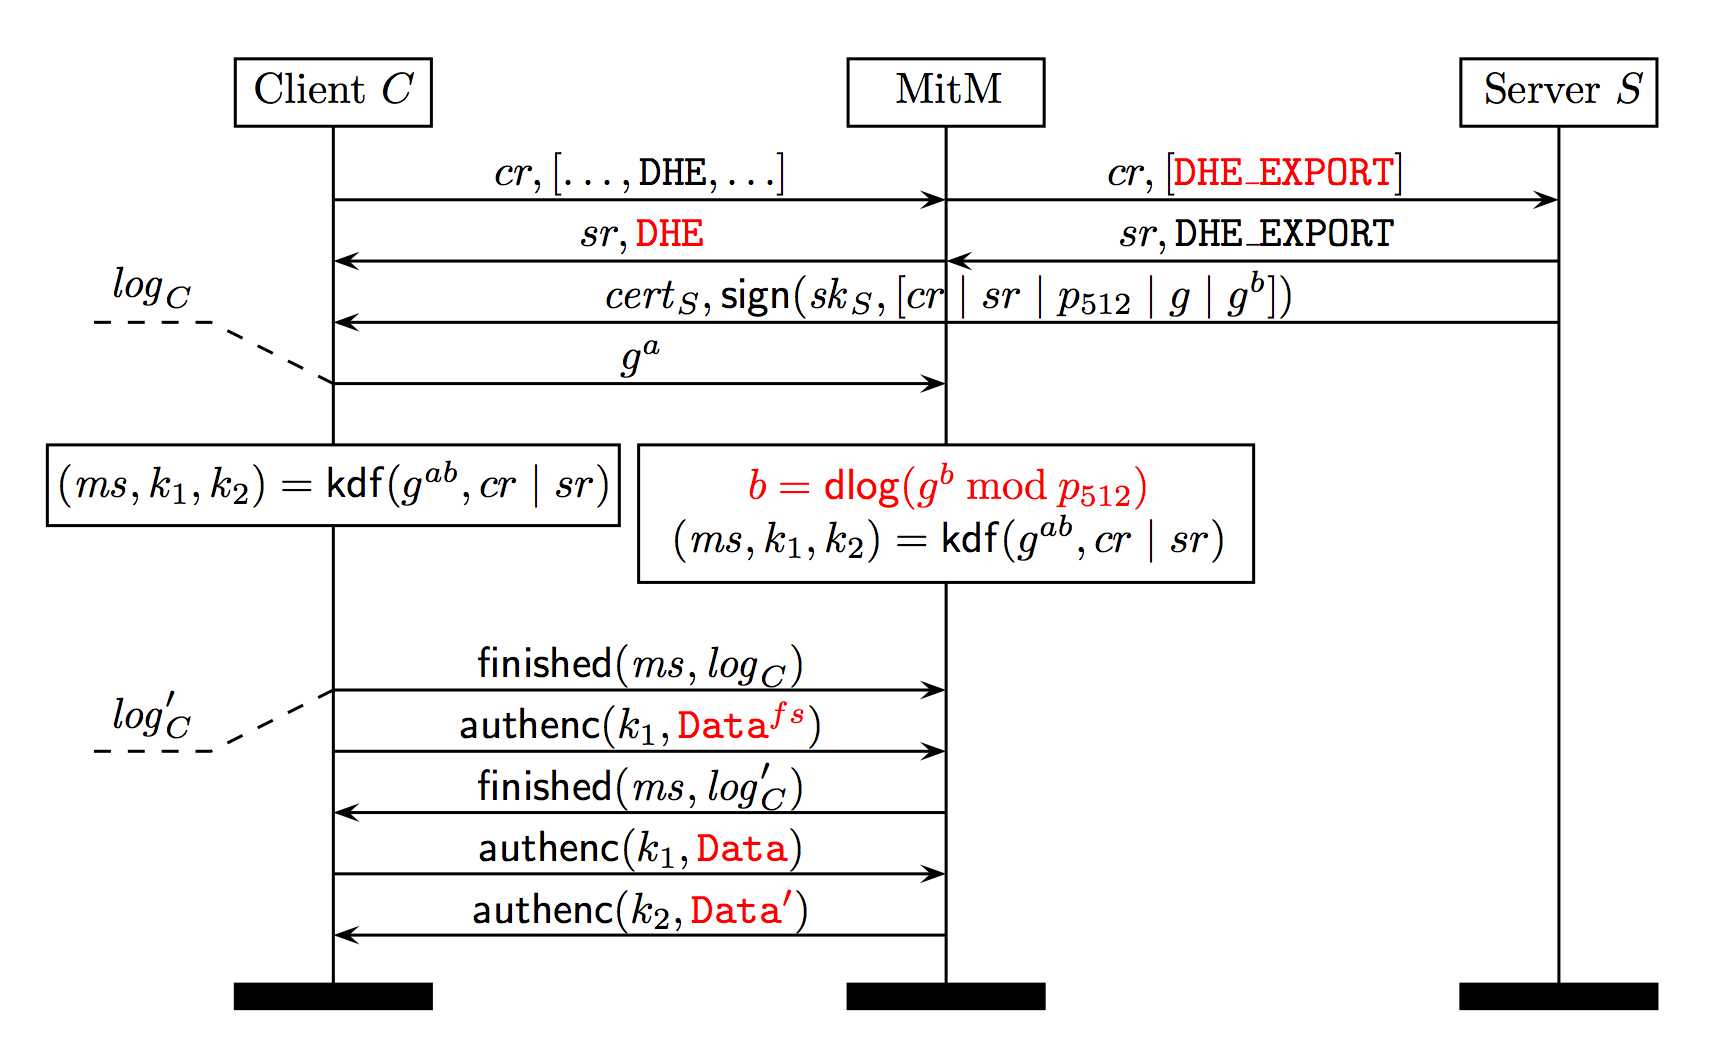
\includegraphics[width=\linewidth]{\LogjamFigures/mitm-dhe-export}
    \caption{\textbf{The Logjam attack}\,---\,%
    A man-in-the-middle can force TLS clients to use export-strength DH with
    any server that allows \dheexp{}. Then, by finding the 512-bit discrete
    log, the attacker can learn the session key and arbitrarily read or
    modify the contents. $\AData^{fs}$ refers to False Start application data
    that some TLS clients send before receiving the server's
    \textsf{Finished} message.}
    \label{fig:mitm-export}
\end{figure}

Given the widespread use of these primes, an attacker with the ability to
compute discrete logs in 512-bit groups could efficiently break \dheexp{}
handshakes for about 8\% of Alexa Top~1M HTTPS sites, but modern browsers
never negotiate export-grade ciphersuites. To circumvent this, we show how an
attacker can downgrade a regular \dhe{} connection to use a \dheexp{} group,
and thereby break both the confidentiality and integrity of application data.

The attack, which we call Logjam, is depicted in Figure~\ref{fig:mitm-export}
and relies on a flaw in the way TLS composes \dhe{} and \dheexp{}. When a
server selects \dheexp{} for a handshake, it proceeds by issuing a signed
\textsf{ServerKeyExchange} message containing a 512-bit $p_{512}$, but the
structure of this message is identical to the message sent during standard
\dhe{} ciphersuites. Critically, the signed portion of the server's message
fails to include any indication of the specific ciphersuite that the server
has chosen. Provided that a client offers \dhe{}, an active attacker can
rewrite the client's \textsf{ClientHello} to offer a corresponding \dheexp{}
ciphersuite accepted by the server and remove other ciphersuites that could
be chosen instead. The attacker rewrites the \textsf{ServerHello} response to
replace the chosen \dheexp{} ciphersuite with a matching non-export
ciphersuite and forwards the \textsf{ServerKeyExchange} message to the client
as is. The client will interpret the export-grade tuple $(p_{512}, g, g^b)$
as valid \dhe{} parameters chosen by the server and proceed with the
handshake. The client and server have different handshake transcripts at this
stage, but an attacker who can compute $b$ in close to real time can then
derive the master secret and connection keys to complete the handshake with
the client.

There are two remaining challenges in implementing this active downgrade
attack. The first is to compute individual discrete logs in close to real
time, and the second is to delay handshake completion until the discrete log
computation has had time to finish.

\subsection{512-bit Discrete Log Computations}
\label{subsec:512bit-dl-computation}

We modified CADO-NFS~\cite{cado-nfs-2.3} to implement the number field sieve
discrete log algorithm and applied it to the top two \dheexp{} primes shown
in Table~\ref{tab:export-primes}. Precomputation took 7~days for each prime,
after which computing individual logarithms requires a median of 70~seconds.

\paragraph{Precomputation}
As illustrated in Figure~\ref{fig:nfs}, the precomputation phase includes the
polynomial selection, sieving, and linear algebra steps. For this
precomputation, we deliberately sieved more than strictly necessary. This
enabled two optimizations: first, with more relations obtained from sieving,
we eventually obtain a larger database of known logarithms, which makes the
descent faster. Second, more sieving relations also yield a smaller linear
algebra step, which is desirable because sieving is much easier to
parallelize than linear algebra.
%\looseness=-1

For the polynomial selection and sieving steps, we used idle time on
2000--3000 CPU cores in parallel. Polynomial selection ran for about 3~hours
(7,600 core-hours). Sieving ran for 15~hours (21,400 core-hours). This
sufficed to collect 40\,M relations of which 28\,M were unique, involving
15\,M primes of at most 27~bits.

From this data set, we obtained a square matrix with 2.2\,M rows and columns,
with 113 nonzero coefficients per row on average. We solved the corresponding
linear system on a 36-node cluster using the block Wiedemann
algorithm~\cite{coppersmith-block-wiedemann-1994,thome-block-wiedemann-2002}.
Using unoptimized code, the computation finished in 120 hours (60,000
core-hours).

The experiment above was done with CADO-NFS in early 2015. As of 2017,
release 2.3 of CADO-NFS~\cite{cado-nfs-2.3} performs 20\% faster for sieving,
and drastically faster for linear algebra, since 9,000 core-hours suffice to
solve the same linear system on the same hardware. In total, the wall-clock
time for each precomputation was slightly over one week in 2015, and is
reduced to about two days with current hardware and more recent software.

\paragraph{Descent}
Once this precomputation was finished, we were able to run the final descent
step to compute individual discrete logs in about a minute. We implemented
the descent calculation in a mix of Python and C\@. On average, computing
individual logarithms took about 70~seconds, but the time varied from 34 to
206 seconds on a server with two 18-core Intel Xeon E5-2699 CPUs. For
purposes of comparison, a single 512-bit RSA factorization using the CADO-NFS
implementation takes about 4 days of wall-clock time on the computer used for
the descent\cite{cado-nfs-2.3}.

% reference: revision 580f1f1 of CADO-NFS with tasks.sieve.qmin=15470309
% on a catrel node:
% Total cpu/elapsed time for entire factorization: 1.06608e+07/351570
% 351570/3600/24 = 4.07

\subsection{Active Attack Implementation}
The main challenge in performing this attack is to compute the shared secret
$g^{ab}$ before the handshake completes in order to forge a \textsf{Finished}
message from the server. With our descent implementation, the computation
takes an average of 70 seconds, but there are several ways an attacker can
work around this delay:

\paragraph{Non-browser clients}
Different TLS clients impose different time limits, after which they kill the
connection. Command-line clients such as \texttt{curl} and \texttt{git} have
long or no timeouts, and we can hijack their connections without difficulty.

\paragraph{TLS warning alerts}
Web browsers tend to have shorter timeouts, but we can keep their connections
alive by sending TLS warning alerts, which are ignored by the browser but
reset the handshake timer. For example, this allows us to keep Firefox TLS
connections alive indefinitely.

\paragraph{Ephemeral key caching}
Many TLS servers do not use a fresh value $b$ for each connection, but
instead compute $g^b$ once and reuse it for multiple negotiations. For
example, F5 BIG-IP load balancers will reuse $g^b$ by default. Microsoft
Schannel caches $g^b$ for two hours---this setting is hard-coded. For these
servers, an attacker can compute the discrete log of $g^b$ from one
connection and use it to attack later handshakes.

\paragraph{TLS False Start}
Even when clients enforce shorter timeouts and servers do not reuse values
for $b$, the attacker can still break the confidentiality of user requests
that use TLS False Start. Recent versions of Chrome, Internet Explorer, and
Firefox implement False Start, but their policies on when to enable it vary.
Firefox 35, Chrome 41, and Internet Explorer (Windows 10) send False Start
data with \dhe{}\@. In these cases, a man-in-the-middle can record the
handshake and decrypt the False Start payload at leisure.

\section{Nation-State Threats to DH}
\label{sec:nationstate}

The previous sections demonstrate the existence of practical attacks against
Diffie-Hellman key exchange as currently used by TLS\@. However, these
attacks rely on the ability to downgrade connections to export-grade crypto.
In this section we address the following question: how secure is
Diffie-Hellman in broader practice, as used in other protocols that do not
suffer from downgrade, and when applied with stronger groups?

\begin{table*}
\centering\small
\begin{tabular}{rrrrrrl@{}}
\toprule
  & \multicolumn{2}{c}{Sieving} & \multicolumn{2}{c}{Linear Algebra} & \multicolumn{1}{c}{Descent} \\
 \cmidrule(r){2-3} \cmidrule(r){4-5} \cmidrule(){6-6}
 & $\log_2B$ & core-years  & rows & core-years  & core-time   \\
\midrule
% timings below from CADO-NFS revision 580f1f1 on a catrel node
% with tasks.sieve.qmin=15470309
% Info:Lattice Sieving: Total CPU time: 9.53745e+06s -> 0.30 cpu year
% Info:Filtering - Merging: Merged matrix has 4146413 rows and total weight 704890615 (170.0 entries per row on average)
% Info:Linear Algebra: Krylov: WCT time 21706.76
% Info:Linear Algebra: Lingen CPU time 4834.58, WCT time 218.43
% Info:Linear Algebra: Mksol: WCT time 11599.56
% Linear Algebra: total WCT = 33524.75
% thus cpu <= 32*WCT <= 1.072792e6 (32 threads) <= 0.03 cpu year
\multicolumn{1}{r}{RSA-512} &
29 & 0.3 &  4.2M & 0.03 &  
& \scriptsize\quad Timings with default CADO-NFS parameters.\\
\multicolumn{1}{r}{DH-512} &
27& 2.5 &  2.2M & 1.1 &  10\,mins
& \scriptsize\quad For the computations in this paper; may be suboptimal.\\
\cmidrule{1-7}
\multicolumn{1}{r}{RSA-768} & 
37& 800 & 250M & 100 &
& \scriptsize\quad Est.\ based on~\cite{rsa768} with less sieving.  \\
%\multicolumn{1}{r}{DH-768} &
%  35 & 8,000 & 150M & 28,500 & 2\,days
%& \scriptsize\quad Est.\ based on~\cite{rsa768,dlp180} and our own experiments. \\
\multicolumn{1}{r}{DH-768} &
36 & 4,000 & 24M & 920 & 43\,hours
    & \scriptsize\quad Data from~\cite[Table 1]{Kleinjung2017}.\\
\cmidrule{1-7}
\multicolumn{1}{r}{RSA-1024} &
42& $\approx$1,000,000  & $\approx$8.7B & $\approx$120,000 & 
& \scriptsize\quad Crude estimate based on complexity formula. \\
%\multicolumn{1}{r}{DH-1024} &
%   40 & 10,000,000 & 5.2B & 35,000,000 & 30\,days
%& \scriptsize\quad Est.\ based on complexity formula and our experiments. \\
\multicolumn{1}{r}{DH-1024} &
   40 & $\approx$5,000,000 & $\approx$0.8B & $\approx$1,100,000 & 30\,days
& \scriptsize\quad Crude estimate based on formula and our experiments. \\
\bottomrule
\end{tabular}

\caption{\textbf{Estimating costs for factoring and discrete log}.
For sieving, we give one important parameter, which is the number of bits of the
smoothness bound
{\tt B}.
For linear algebra, all costs for DH are for
safe primes; for DSA primes with $q$ of 160 bits, this should be
divided by 6.4 for 1024 bits, 4.8 for 768 bits, and 3.2 for 512 bits.}

\label{tab:costs}
\end{table*}



To answer this question we must first examine how the number field sieve for
discrete log scales to 768- and 1024-bit groups. As we argue below, 768-bit
groups in relatively widespread use are now within reach for academic
computational resources. Additionally, performing precomputations for a small
number of 1024-bit groups is plausibly within the resources of nation-state
adversaries. The precomputation would likely require special-purpose
hardware, but would not require any major algorithmic improvements. In light
of these results, we examine several standard Internet security
protocols---IKE, SSH, and TLS---to determine their vulnerability. Although
the cost of the precomputation for a 1024-bit group is several times higher
than for an RSA key of equal size, a one-time investment could be used to
attack millions of hosts, due to widespread reuse of the most common
Diffie-Hellman parameters. Finally, we apply this new understanding to a set
of recently published documents to evaluate the hypothesis that the National
Security Agency has {\em already} implemented such a capability.

\subsection{Scaling NFS to 768- and 1024-bit DH}

Estimating the cost for discrete log cryptanalysis at larger key sizes is far
from straightforward due to the complexity of parameter tuning. We attempt
estimates up to 1024-bit discrete log based on the existing literature and
our own experiments but further work is needed for greater confidence. We
summarize all the costs, measured or estimated, in Table~\ref{tab:costs}.

\paragraph{DH-768: Completed in 2016}
At the time of disclosure, the latest discrete log record was a 596-bit
computation. Based on that work, and on prior experience with the 768-bit
factorization record in 2009~\cite{factor-rsa-768}, we made the conservative
prediction that it was possible, as explained in~\S\ref{sec:dl}, to put more
computational effort into sieving for the discrete log case than for
factoring, so that the linear algebra step would run on a slightly smaller
matrix. This led to a runtime estimate of around 35,000 core-years, most of
which was spent on linear algebra.

This estimate turned out be overly conservative, for several reasons. First,
there have been significant improvements in our software implementation
(see~\S\ref{subsec:512bit-dl-computation}). In addition, our estimate did not
use the Joux-Lercier alternative polynomial selection
method~\cite[\S2.1]{nfs-prime-field-2003}, which is specific to discrete
logs. For 768-bit discrete logs, this polynomial selection method leads to a
significantly smaller computational cost.

In 2016, Kleinjung et al.\ completed a 768-bit discrete log
computation~\cite{compute-dlog-768}. While this is a massive computation on
the academic scale, a computation of this size has likely been within reach
of nation-states for more than a decade. This data is mentioned in
Table~\ref{tab:costs}.

\paragraph{DH-1024: Plausible with nation-state resources}
Experimentally extrapolating sieving parameters to the 1024-bit case is
difficult due to the tradeoffs between the steps of the algorithm and their
relative parallelism. The prior work proposing parameters for factoring a
1024-bit RSA key is thin and we resort to extrapolating from asymptotic
complexity. For the number field sieve, the complexity is
$\exp\big((k+o(1))(\log N)^{1/3}(\log\log N)^{2/3}\big),$ where $N$ is the
integer to factor or the prime modulus for discrete log and $k$ is an
algorithm-specific constant. This formula is inherently imprecise, since the
$o(1)$ in the exponent can hide polynomial factors. This complexity formula,
with $k=1.923$, describes the overall time for both discrete log and
factorization, which are both dominated by sieving and linear algebra in the
precomputation. Evaluating the formula for 768- and 1024-bit $N$ gives us
estimated multiplicative factors by which time and space will increase from
the 768- to the 1024-bit case.

For 1024-bit precomputation, the total time complexity can be expected to
increase by a factor of 1220 using the complexity formula, while space
complexity increases by its square root, approximately 35. These ratios are
relevant for both factorization and discrete log since they have the same
asymptotic behavior. For DH-1024, we get a total cost estimate for the
precomputation of about 6M core-years.

The time complexity for each individual log after the precomputation should
be multiplied by $L_{2^{1024}}(1.206)/L_{2^{768}}(1.206)\approx86$, where
$k=1.206$ follows from~\cite{hidden-snfs-1024-2017}. This last number does
not correspond to what we observed in practice and we attribute that to the
fact that the descent step has been far less studied.

In practice, it is not uncommon for estimates based merely on the complexity
formula to be off by a factor of 10. Estimates of Table~\ref{tab:costs} must
therefore be considered with due caution.

For 1024-bit descent, we experimented with our early-abort implementation to
inform our estimates for descent initialization, which should dominate the
individual discrete log computation. For a random target in Oakley Group~2,
initialization took 22 core-days, and yielded a few primes of at most 130
bits to be descended further. In twice this time, we reached primes of about
110 bits. At this point, we were certain to have bootstrapped the descent and
could continue down to the smoothness bound in a few more core-days if proper
sieving software were available. Thus we estimate that a 1024-bit descent
would take about 30~core-days, once again easily parallelizable.

\paragraph{Costs in hardware}
Although several millions of core-years is a massive computational effort, it
is not necessarily out of reach for a nation-state. At this scale,
significant cost savings could be realized by developing application-specific
hardware given that sieving is a natural target for hardware implementation.
To our knowledge, the best prior description of an ASIC implementation of
1024-bit sieving is the 2007 work of Geiselmann and
Steinwandt~\cite{hardware-scaling-nfs-2007}. Updating their estimates for
modern techniques and adjusting parameters for discrete log allows us to
extrapolate the financial and time costs.

We increase their chip count by a factor of ten to sieve more and save on
linear algebra as above giving an estimate of 3M chips to complete sieving in
one year. Shrinking the dies from the 130~nm technology node used in the
paper to a more modern size reduces costs as transistors are cheaper at newer
technologies. With standard transistor costs and utilization, it would cost
about \$2 per chip to manufacture after fixed design and tape-out costs of
roughly \$2M~\cite{jefferies-report-2012}. This suggests that an \$8M
investment would buy enough ASICs to complete the DH-1024 sieving
precomputation in one year. Since a step of descent uses sieving, the same
hardware could likely be reused to speed calculations of individual
logarithms.

Estimating the financial cost for the linear algebra is more difficult since
there has been little work on designing chips that are suitable for the
larger fields involved in discrete log. To derive a rough estimate, we can
begin with general purpose hardware and the core-year estimate from
Table~\ref{tab:costs}. Using the 300,000 CPU core Titan supercomputer it
would take 4~years to complete the 1024-bit linear algebra stage
(notwithstanding the fact that estimates from Table~\ref{tab:costs} are known
to be extremely coarse, and could be optimistic by a factor of maybe 10).
Titan was constructed in 2012 for \$94M, suggesting a cost of \$0.5B in
supercomputers to finish this step in a year. In the context of
factorization, moving linear algebra from general purpose CPUs to ASICs has
been estimated to reduce costs by a factor of
80~\cite{improving-linear-algebra-nfs-2005}. If we optimistically assume that
a similar reduction can be achieved for discrete log, the hardware cost to
perform the linear algebra for DH-1024 in one year is plausibly on the order
of tens of millions of dollars.

To put this dollar figure in context, the FY\,2012 budget for the U.S.
Consolidated Cryptologic Program (which includes the NSA) was \$10.5
billion\footnote{\small The National Science Foundation's budget was \$7
billion.}~\cite{black-budget-leak-2013}. The 2013 budget request, which
prioritized investment in ``groundbreaking cryptanalytic capabilities to
defeat adversarial cryptography and exploit internet traffic'' included
notable \$100M+ increases in two programs under Cryptanalysis \& Exploitation
Services: ``Cryptanalytic IT Systems'' (to \$247M), and the cryptically named
``PEO Program C'' (to \$360M)~\cite{black-budget-leak-2013}.

\subsection{Is NSA Breaking 1024-bit DH?}

Our calculations suggest that it is plausibly within NSA's resources to have
performed number field sieve precomputations for a small number of 1024-bit
Diffie-Hellman groups. This would allow them to break any key exchanges made
with those groups in close to real time. If true, this would answer one of
the major cryptographic questions raised by the Edward Snowden leaks: How is
NSA defeating the encryption for widely used VPN protocols?

Virtual private networks (VPNs) are widely used for tunneling business or
personal traffic across potentially hostile networks. We focus on the
Internet Protocol Security (IPsec) VPN protocol using the Internet Key
Exchange (IKE) protocol for key establishment and parameter negotiation and
the Encapsulating Security Payload (ESP) protocol for protecting packet
contents.

\paragraph{IKE}
There are two versions, IKEv1 and IKEv2, which differ in message structure
but are conceptually similar. For the sake of brevity, we will use IKEv1
terminology~\cite{rfc7296}.

\newcommand{\skeyid}{\textsf{\small SKEYID}}
\newcommand{\keymat}{\textsf{\small KEYMAT}}
\newcommand{\psk}{\textsf{\small PSK}}

Each IKE session begins with a Phase~1 handshake in which the client and
server select a Diffie-Hellman group from a small set of standardized
parameters and perform a key exchange to establish a shared secret. The
shared secret is combined with other cleartext values transmitted by each
side, such as nonces and cookies, to derive a value called \skeyid\@. When
authenticated with a pre-shared key (PSK) in IKEv1, the PSK value is
incorporated into the derivation of \skeyid.

The resulting \skeyid\ is used to encrypt and authenticate a Phase~2
handshake. Phase~2 establishes the parameters and key material, \keymat, for
protecting the subsequently tunneled traffic. Ultimately, \keymat{} is
derived from \skeyid, additional nonces, and the result of an optional
Phase~2 Diffie-Hellman exchange.

\paragraph{NSA's VPN exploitation process}
Documents published by Der Spiegel describe NSA's ability to decrypt VPN
traffic using passive eavesdropping and without message injection or
man-in-the-middle attacks on IPsec or IKE\@. Figure~\ref{fig:scarynsafigure}
illustrates the flow of information required to decrypt the tunneled traffic.

\begin{figure}
    \noindent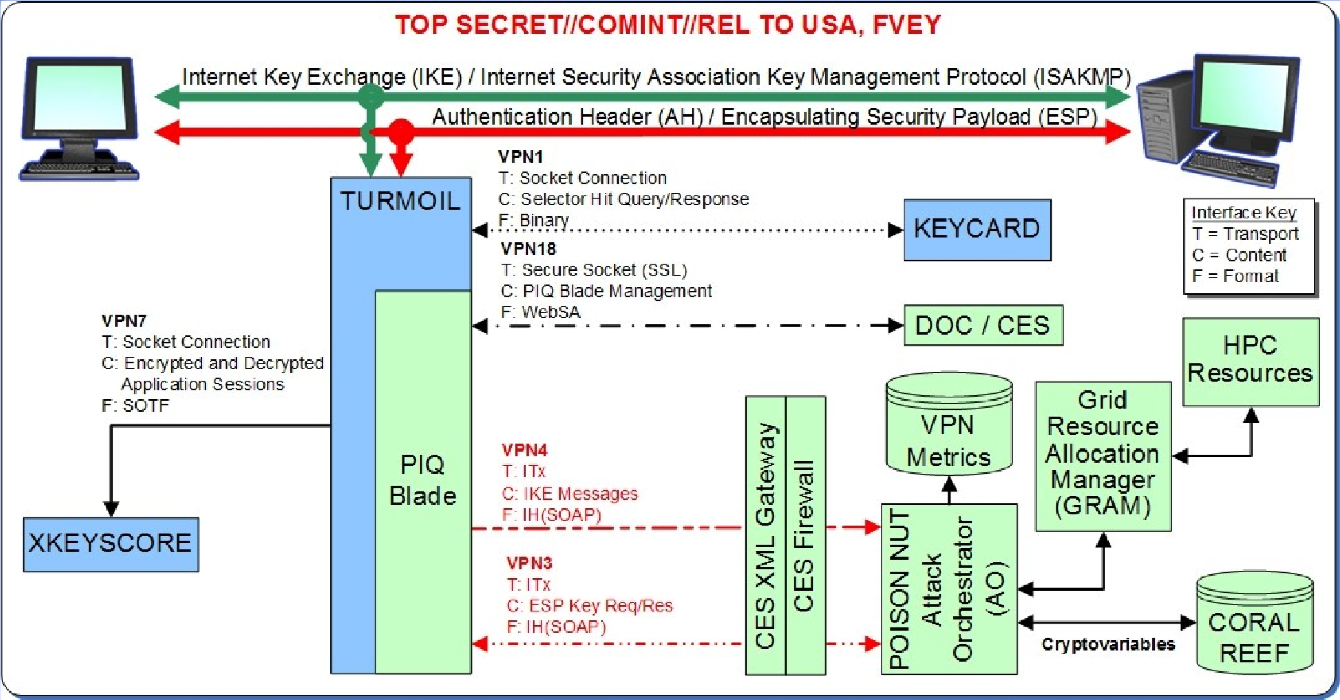
\includegraphics[width=\linewidth]{\LogjamFigures/NSA_combined.png}
    \caption{\textbf{NSA's VPN decryption infrastructure}\,---\,%
    This classified illustration published by Der
    Spiegel~\cite{media-35526} shows captured IKE handshake messages
    being passed to a high-performance computing system, which returns the
    symmetric keys for ESP session traffic. The details of this attack are
    consistent with an efficient break for 1024-bit Diffie-Hellman.}
    \label{fig:scarynsafigure}
\end{figure}

\begin{table*}[t]
\small
\centering
\begin{tabular}{lrrrr}
\toprule
              & \multicolumn{4}{c}{\emph{Vulnerable servers, if the attacker can precompute for \ldots}} \\
\cmidrule{2-5}
%\multicolumn{1}{r}{\emph{If the attacker can precompute \ldots.}}
              & all 512-bit groups & all 768-bit groups & one 1024-bit group & ten 1024-bit groups\\  
\midrule
HTTPS Top~1M w/ active downgrade\qquad\strut & 45,100 (8.4\%) & 45,100 (8.4\%) & 205,000 (37.1\%) & 309,000 (56.1\%) \\
HTTPS Top~1M & 118 (0.0\%) & 407 (0.1\%) & 98,500 (17.9\%) & 132,000 (24.0\%) \\
HTTPS Trusted w/ active downgrade & 489,000 (3.4\%) & 556,000 (3.9\%) & 1,840,000 (12.8\%) & 3,410,000 (23.8\%) \\ 
HTTPS Trusted &  1,000 (0.0\%) & 46,700 (0.3\%) & 939,000 (6.56\%) & 1,430,000 (10.0\%)\medskip\\
IKEv1 IPv4  & -- & 64,700 (2.6\%) & 1,690,000 (66.1\%)& 1,690,000 (66.1\%) \\
IKEv2 IPv4  & -- & 66,000 (5.8\%) & 726,000 (63.9\%) & 726,000 (63.9\%)\medskip \\
SSH   IPv4  & -- & -- & 3,600,000 (25.7\%) & 3,600,000 (25.7\%) \\
\bottomrule

\end{tabular}
\caption{\textbf{Estimated impact of Diffie-Hellman attacks in early 2015.}
We used Internet-wide scanning to estimate the number of real-world servers for which 
typical connections could be compromised by attackers with various levels of computational
resources. For HTTPS, we provide figures with and without downgrade attacks on the chosen ciphersuite. All others are passive attacks.
}
\end{table*}


When the IKE/ESP messages of a VPN of interest are collected, the IKE
messages and a small amount of ESP traffic are sent to the Cryptanalysis and
Exploitation Services (CES)~\cite{media-35526,media-35529,media-35515}.
Within the CES enclave, a specialized ``attack orchestrator'' attempts to
recover the ESP decryption key with assistance from high-performance
computing resources as well as a database of known PSKs
(``CORALREEF'')~\cite{media-35529,media-35526,media-35515}. If the recovery
was successful, the decryption key is returned from CES and used to decrypt
the buffered ESP traffic such that the encapsulated content can be
processed~\cite{media-35529,media-35522}.

\paragraph{Evidence for a discrete log attack}
The ability to decrypt VPN traffic does not necessarily indicate a defeat of
Diffie-Hellman. There are, however, several features of the described
exploitation process that support this hypothesis.

The IKE protocol has been extensively
analyzed~\cite{ike-security-2002,ike-nrl-1999} and is not believed to be
exploitable in standard configurations under passive eavesdropping attacks.
Absent a vulnerability in the key derivation function or transport
encryption, the attacker must recover the decryption keys. This requires the
attacker to calculate \skeyid{} generated from the Phase~1 Diffie-Hellman
shared secret after passively observing an IKE handshake.

While IKE is designed to support a range of Diffie-Hellman groups, our
Internet-wide scans (\S\ref{sec:1024effects}) show that the vast majority of
IKE endpoints select one particular 1024-bit DH group even when offered
stronger groups. Conducting an expensive, but feasible, precomputation for
this single 1024-bit group (Oakley Group 2) would allow the efficient
recovery of a large number of Diffie-Hellman shared secrets used to derive
\skeyid{} and the subsequent \keymat.

Given an efficient oracle for solving the discrete logarithm problem, attacks
on IKE are possible provided that the attacker can obtain the following:
$(1)$ a complete two-sided IKE transcript, and $(2)$ any PSK used for
deriving {\skeyid} in IKEv1. The available documents describe both of these
as explicit prerequisites for the VPN exploitation process outlined above and
provide the reader with internal resources available to meet these
prerequisites~\cite{media-35515}.

Of course, this explanation is not dispositive and the possibility remains
that NSA could defeat VPN encryption using alternative means. A published NSA
document refers to the use of a router ``implant'' to allow decryption of
IPsec traffic indicating that the use of targeted malware is possible. This
implant ``allows passive exploitation with just ESP''~\cite{media-35515}
without the prerequisite of collecting the IKE handshake messages. This
indicates that it is an alternative mechanism to the attack described above.

The most compelling argument for a pure cryptographic attack is the
generality of the NSA's VPN exploitation process. This process appears to be
applicable across a broad swath of VPNs without regard to endpoint's identity
or the ability to compromise individual endpoints.


\subsection{Effects of a 1024-bit Break}
\label{sec:1024effects}

In this section, we use Internet-wide scanning to assess the impact of a
hypothetical DH-1024 break on IKE, SSH, and HTTPS\@. Our measurements,
performed in early 2015, indicate that these protocols would be subject to
widespread compromise by a nation-state attacker who had the resources to
invest in precomputation for a small number of 1024-bit groups.

\paragraph{IKE}
We measured how IPsec VPNs use Diffie-Hellman in practice by scanning a 1\%
random sample of the public IPv4 address space for IKEv1 and IKEv2 (the
protocols used to initiate an IPsec VPN connection) in May~2015. We used the
ZMap UDP probe module to measure support for Oakley Groups~1 and~2 (two
popular 768- and 1024-bit, built-in groups) and which group servers prefer.
Of the 80K hosts that responded with a valid IKE packet, 44.2\% were willing
to negotiate a connection using one of the two groups. We found that 31.8\%
of IKEv1 and 19.7\% of IKEv2 servers support Oakley Group~1 (768-bit) while
86.1\% and 91.0\% respectively supported Oakley Group~2 (1024-bit). In our
sample of IKEv1 servers, 2.6\% of profiled servers preferred the 768-bit
Oakley Group~1 and 66.1\% preferred the 1024-bit Oakley Group~2. For IKEv2,
5.8\% of profiled servers chose Oakley Group~1, and 63.9\% chose Oakley
Group~2.

\paragraph{SSH}
All SSH handshakes complete either a finite field or elliptic curve
Diffie-Hellman exchange. The protocol explicitly defines support for Oakley
Group~2 (1024-bit) and Oakley Group~14 (2048-bit) but also allows a
server-defined group to be negotiated. We scanned 1\% random samples of the
public IPv4 address space in April 2015. We find that 98.9\% of SSH servers
support the 1024-bit Oakley Group~2, 77.6\% support the 2048-bit Oakley
Group~14, and 68.7\% support a server-defined group\@.

During the SSH handshake, the server selects the client's highest priority
mutually supported key exchange algorithm. To estimate what servers will
prefer in practice, we performed a scan in which we mimicked the algorithms
offered by OpenSSH 6.6.1p1, the latest version of OpenSSH\@. In this scan,
21.8\% of servers preferred the 1024-bit Oakley Group~2, and 37.4\% preferred
a server-defined group. 10\% of the server-defined groups were 1024-bit, but,
of those, nearly all provided Oakley Group~2 rather than a custom group.

Combining these equivalent choices, we find that a nation-state adversary who
performed NFS precomputations for the 1024-bit Oakley Group~2 could passively
eavesdrop on connections to 3.6M (25.7\%) publicly accessible SSH servers.

\paragraph{HTTPS}
\dhe is commonly deployed on web servers. 68.3\% of Alexa Top~1M sites
support \dhe, as do 23.9\% of sites with browser-trusted certificates. Of the
Top~1M sites that support \dhe, 84\% use a 1024-bit or smaller group, with
94\% of these using one of five groups.

Despite widespread support for \dhe, a passive eavesdropper can only decrypt
connections that organically agree to use Diffie-Hellman. We estimate the
number of sites for which this will occur by offering the same sets of
ciphersuites as Chrome, Firefox, and Safari. Approximately 24.0\% of browser
connections with HTTPS-enabled Top~1M sites (and 10\% with browser-trusted
sites) will negotiate \dhe with one of the ten most popular 1024-bit primes;
17.9\% of connections with Top~1M sites could be passively eavesdropped given
the precomputation for a single 1024-bit prime.


\section{Recommendations}
\label{sec:lessons}

In this section, we present concrete recommendations to recover the expected
security of Diffie-Hellman.

\paragraph{Transition to elliptic curves.}
Transitioning to elliptic curve Diffie-Hellman (ECDH) key exchange avoids all
known feasible cryptanalytic attacks. Current elliptic curve discrete log
algorithms do not gain as much of an advantage from precomputation. In
addition, ECDH keys are shorter and computations are faster. We recommend
transitioning to elliptic curves; this is the most effective solution to the
vulnerabilities in this paper. We note that in August 2015, the NSA announced
that it was planning to transition away from elliptic curve cryptography for
its Suite B cryptographic algorithms and would replace them with algorithms
resistant to quantum computers~\cite{nsa-suiteb}. However, since no fully
vetted and standardized quantum-resistant algorithms exist currently,
elliptic curves remain the most secure choice for public key operations.

\paragraph{Increase minimum key strengths.}
To protect against the Logjam attack, server operators should disable \dheexp
and configure \dhe ciphersuites to use primes of 2048 bits or larger.
Browsers and clients should raise the minimum accepted size for
Diffie-Hellman groups to at least 1024 bits in order to avoid downgrade
attacks.

\paragraph{Don't deliberately weaken crypto.}
The Logjam attack illustrates the fragility of cryptographic ``front doors''.
Although the key sizes originally used in \dheexp were intended to be
tractable only to NSA, two decades of algorithmic and computational
improvements have significantly lowered the bar to attacks on such key sizes.
Despite the eventual relaxation of crypto export restrictions and subsequent
attempts to remove support for \dheexp{}, the technical debt induced by the
additional complexity has left implementations vulnerable for decades. Like
FREAK~\cite{freak-attack-2015}, our attacks warn of the long-term
debilitating effects of deliberately weakening cryptography.


\section{Conclusion}
\label{sec:conclusion}

We find that Diffie-Hellman key exchange, as used in practice, is often less
secure than widely believed. The problems stem from the fact that the number
field sieve for discrete log allows an attacker to perform a single
precomputation that depends only on the group, after which computing
individual logarithms in that group has a far lower cost. Although this is
well known to cryptographers, it apparently has not been widely understood by
system builders. Likewise, many cryptographers did not appreciate that a
large fraction of Internet communication depends on a few small, widely
shared groups.
%\looseness=-1

A key lesson is that cryptographers and creators of practical systems need to
work together more effectively. System builders should take responsibility
for being aware of applicable cryptanalytic attacks. Cryptographers should
involve themselves in how crypto is actually being applied, such as through
engagement with standards efforts and software review. Bridging the perilous
gap that separates these communities will be essential for keeping future
systems secure.

%\section*{Acknowledgments}
%
%The authors thank Michael Bailey, Daniel Bernstein, Ron Dreslinski,
%Tanja Lange, Adam Langley, Kenny Paterson, Andrei Popov, Ivan Ristic,
%Edward Snowden, Brian Smith, Martin Thomson, and Eric Rescorla.  This
%work was supported by the U.S. National Science Foundation, the Office
%of Naval Research, the European Research Council, and the French
%National Research Agency, with additional support from the Mozilla
%Foundation, Supermicro, Google, Cisco, the Morris Wellman
%Professorship, and the Alfred P. Sloan Foundation.  Some experiments
%used the Grid'5000 testbed, supported by INRIA, CNRS, RENATER, and
%others.
